\section{Evaluation}
\label{SEC:evaluation}

Satisfied that we had a implementation of AES our efforts turned to
demonstrating that it could effectively test real world applications.  To
this end, we extensively evaluated CrashSimulator against a variety of
applications and anomalies in a laboratory environment.
Additionally, we conducted a user study in which undergraduate and
graduate computer science students got a chance to test applications of
their choosing using CrashSimulator with the goal of identifying new bugs
and reporting to the application's developers.
We used the results from both these efforts to answer the following questions:

\begin{enumerate}

\item{Is CrashSimulator able to identify a wide variety of environmental
    bugs?
(Subsection~\ref{sec-env-bugs})}

\item{Do tests using CrashSimulator make yield too many false positives?
      (Subsection~\ref{sec-sorts-errors})}

\item{Can CrashSimulator
      execute tests efficiently? (Subsection~\ref{sec-perf})}

\end{enumerate}

\subsection{Is CrashSimulator able to identify a wide variety of
environmental bugs?}
\label{sec-env-bugs}

The most crucial question to ask about CrashSimulator is how readily it can
identify environmental bugs from a wide variety of causes.  To evaluate the
tool in this regard we configured it  to look for bugs from the
categories discussed in Section~\ref{SEC:background}.  These included
bugs related to unusual filesystem conditions and network situations under
Linux.
All of these bugs relied on common sysem calls, and thus had the potential to
appear in many programs.  We selected the tested applications either
because they were deemed ``popular'' by Debian's Popularity
Contest~\cite{DebPopCon}, or were from GNU Coreutils.  Coreutils
applications were chosen because of their widespread inclusion in many
Linux distributions.


\subsubsection{Bugs Related to Moving Files}

As was discussed in Section~\ref{SEC:approach}, the first bug finding
opportunity offered by AES occurs through analyzing an applications unmodified
system call behavior.  To evaluate CrashSimulator's ability to find bugs at
this point, we decided to test applications that move files
about on the filesystem.  In many cases this operation can be handled
atomically by the operating system through the {\tt rename()} system call.
However, in situations where the source file and destination file are on
different storage devices, the application must
manually perform all of the required steps.
This is an process that even well-tested applications
frequently get wrong~\cite{PHPRenameBug,PythonShutilBug,NodejsCopyBug}.

{\bf Method.}  Catching this particular bug requires CrashSimulator to use
checkers that encodes the correct steps involved in moving a file from one
storage device to another. To identify these steps
we examined several libraries and applications and found that {\tt mv} seemed
to handle cases that other tools failed to consider.  Following this, we
used its behavior as a template to create a set of checkers that
evaluate whether or not the application performs the following
checks and operations:

\paragraph{Source Replaced}

An application should make an effort to ensure that the file being copied is not
replaced between the time it is initially examined and the time it is opened
for copying.  Otherwise it could have been replaced by a file of a different
type, such as a character device.
To test whether applications are robust to anomalies involving source file replacement,
we developed a checker that monitors whether a series of safety checks
are performed.
Failing to perform these checks often results in corruption of the file~\cite{PythonShutilBug}.

\paragraph{Preserve Xattrs}

Extended file attributes are used by modern
operating systems to store descriptive information about a file that cannot be
held by normal filesystem fields.  For example, an operating system can use
extended file attributes to record whether or not a file was downloaded from the
Internet -- important security information that is used to warn
users if they are about to open a potentially unsafe file.  Apple's Gatekeeper
relies on extended file attributes to prevent the execution of applications downloaded from
untrusted developers without explicit user action~\cite{AppleCodeSigning}.
When copying a file,
an application should retrieve extended file attributes from the source
file and, later, apply them to the destination file.
In this case, CrashSimulator used a checker
that watches for the application to make system calls
that read the extended file attributes from the source file (i.e. {\tt
  getxattr()}, {\tt lgetxattr()}, or {\tt fgetxattr()}) followed by system calls
that re-apply the attributes to the destination file (i.e. {\tt setxattr()},
{\tt lsetxattr()}, or {\tt fsetxattr()}).

\paragraph{Preserve Timestamps}

In order to truly copy a file from one device
to another an application needs to ensure that its metadata (such as the
creation, modification, and access times) are preserved in the destination
file.
In this case, the checker monitors
whether the application applies
the appropriate timestamps to the destination file as part of moving a file
across devices by monitoring for a system call from the {\tt stat()} family to
retrieve the timestamps and system call from the {\tt utime()} family to apply
the retrieved timestamps to the destination file.
Failure to preserve timestamps has obvious
implications in records-keeping and archival situations as well as any situation
where a chronological record of file manipulations is important.  This can
cause odd behavior in Makefiles, archival programs, and similar
software~\cite{NautilusTimestamps, SudoTimestamp}.

\paragraph{Copying Devices}

It is also important to check if a move would attempt to copy a special
character file like {\tt /dev/urandom} across disks.
Many applications fail to examine the nature of a file before
operating on it.  So the file must be moved by creating a new device of the same
type at the destination, instead of reading from a potentially infinite device.
In our experience, applications that fail to perform this check end up
completely filling a disk or exhausting available memory -- sometimes causing the
system to become unresponsive.


 \begin{table}[t]
    \scriptsize{}
    \begin{tabular}{l p{1cm} p{1cm} p{1.2cm} p{1cm}}
    \toprule{}
        Application     & Source Replaced & Preserve Xattrs & Preserve Timestamps & Copying Devices\\
\hline
        {\tt mv}              & Correct             & Correct         & Correct             & Correct\\
        {\tt mmv}             & Correct             & {\bf Sec. Flaw} & {\bf Time Loss} & Correct\\
        {\tt install}         & Correct             & {\bf Sec. Flaw} & {\bf Time Loss} & {\bf Fill Disk} \\
        {\tt perl File::Copy} & Correct             & {\bf Sec. Flaw} & {\bf Time Loss} & {\bf Fill Disk} \\
        {\tt shutils}         & {\bf Corrupt}	& {\bf Sec. Flaw} 	& Correct             & Correct\\
        {\tt rust}             & Correct             & {\bf Sec. Flaw} & {\bf Time Loss} & {\bf Fill Disk} \\
        {\tt boost::copyfile} & {\bf Corrupt}	      & {\bf Sec. Flaw} & {\bf Time Loss} & {\bf Fill Disk} \\
    \bottomrule{}
    \end{tabular}
    \caption{Applications and libraries analyzed to determine whether or not
      they are able to correctly move a file from one device to another.
Incorrect entries are either missing the needed check or were ineffective.}
    \label{table:crossdevice}
\end{table}

{\bf Findings.}
As can be seen from the results in Table~\ref{table:crossdevice}, each of the
applications tested fails to perform one or more of the steps required to
successfully complete a cross-device move.  This is an unfortunate situation
because a failure to perform any one of these steps can result in negative
outcomes for the system as a whole.
Our results indicate that CrashSimulator is able to identify whether complex
operations are performed correctly in anomalous situations in
an array of popular programs.
This includes the standard libraries for the programming languages Python,
Perl, and Rust, along with other widely used software.  This is true even
when many libraries have correct behavior in some cases, but not others.


\subsubsection{Unexpected File Types}
\label{sec-file-type-bugs}

CrashSimulator's ability
to inject anomalous situations into an application
provides a second opportunity to identify bugs.
To test
its capabilities
at this point we needed
an anomaly
that arises during a common situation --
a Linux application retrieving
and processing data from a file.  Linux supports several special file
types other than the standard ``regular'' file type.
These types include
directories,
symbolic links,
character devices,
block devices,
sockets, and
First-In-First-Out (FIFO) pipes.
While these special files
use the same system calls as regular files (such as {\tt read()} and
{\tt write()}), they behave in very different ways.  For example, {\tt
/dev/urandom} is a character device that produces an infinite amount of
pseudo-random data when read.  If an application that reads the full
contents of a file before processing it is provided {\tt /dev/urandom}, it
will fill memory or disk space and could
crash the system~\cite{YumAptEndless}.
Correct execution in these situations often requires applications
to examine the files in order to ensure they are of an appropriate type.

{\bf Method.}  Identifying these bugs involves changing an application's
execution to induce its response to an unexpected file type.  For
example, the {\tt sed} application, which modifies the contents of a text
file according to a provided command string, could be provided a symbolic
link, a directory, or a character device instead.  CrashSimulator
accomplishes this by identifying the calls to {\tt stat()}, {\tt fstat()},
or {\tt lstat()} that an application makes to examine the file, and then
changes their results to simulate
one of the special file types.  If the application responds to
this injected information then there is the possibility that the special
file will be handled correctly.  On the other hand, if there is no
alteration in the behavior of the application,  then the condition is not
being handled correctly.

{\bf Findings.}
The results of this round of tests were shown in
Table~\ref{table:unexpectedtypes}.

For each application,
CrashSimulator was configured to simulate all of the non-standard file
types.
Table~\ref{table:unexpectedtypes} also shows the values that CrashSimulator
inserted into the results of the {\tt stat()}-like calls made by the
application.
A result of ``Initial Value'' indicates
that this is the file type the application was provided
when the application was initially recorded -- that is,
a file of the type the application was expecting.
A result of ``Recognizes'' indicates that the application
identified that it was being provided with an unexpected file type and its
execution diverged,
indicating that it was potentially handling the
unexpected file type correctly.
A result of ``Fail'' indicates that the
application failed to recognize the presence of the unusual file type
because execution never diverged from the trace being replayed.
We manually examined a subset of the listed application behaviors simulated by
CrashSimulator and verified they were consistent with the actual behavior
on the given file type.

\begin{table*}[t]
    \scriptsize{}
    \begin{tabular}{l  l  |  l  l  l  l  l  l  l}
    \toprule{}
Application & Condition Tested           & IFREG        & IFDIR        &
        IFCHR     & IFBLK    & IFIFO      & IFLNK    & IFSOCK\\
\hline
        {\tt Aspell}      & Dictionary File            & Initial Value  & Fail           & Recognizes  & Fail       & Fail        & Fail       & Fail\\
        {\tt Aspell}      & File being checked         & Initial Value  & Fail           & Recognizes  & Fail       & Fail        & Fail       & Fail\\
        {\tt gnu-gpg}     & secring.gpg                & Initial Value  & Fail           & Fail        & Fail       & Fail        & Fail       & Fail\\
        {\tt vim}         & File being opened          & Initial Value  & Recognizes     & Recognizes  & Recognizes & Recognizes & Recognizes & Fail\\
        {\tt nano}        & File being opened          & Initial Value  & Recognizes     & Recognizes  & Recognizes & Fail        & Fail       & Fail\\
        {\tt sed}         & File being edited          & Initial Value  & Fail           & Recognizes  & Fail       & Fail        & Fail       & Fail\\
        {\tt df}          & /proc                      & Fail           & Initial Value  & Fail        & Fail       & Fail        & Fail       & Fail\\
        {\tt wc}          & File being checked         & Initial Value  & Recognizes     & Recognizes  & Recognizes & Recognizes  & Recognizes & Recognizes\\
        {\tt du}          & Directory being checked    & Recognizes     & Initial Value  & Recognizes  & Recognizes & Recognizes  & Recognizes & Recognizes\\
        {\tt install}     & File being installed       & Initial Value  & Recognizes     & Fail       & Fail      & Fail       & Recognizes & Fail\\
        {\tt fmt}         & File being formatted       & Initial Value  & Fail          & Recognizes  & Fail      & Fail       & Fail      & Fail\\
        {\tt od}          & File being dumped          & Initial Value  & Fail          & Recognizes  & Fail      & Fail       & Fail      & Fail\\
        {\tt ptx}         & File being read            & Initial Value  & Recognizes     & Recognizes  & Recognizes & Recognizes  & Recognizes & Recognizes\\
        {\tt comm}        & Second file being compared & Initial Value  & Fail           & Recognizes  & Fail       & Fail        & Fail       & Fail\\
        {\tt pr}          & File being read            & Initial Value  & Fail           & Fail        & Fail       & Fail        & Fail       & Fail\\
\hline
        {\tt readlink}    & Link being evaluated       & \textbf{No file checks performed} & & & & & & \\
        {\tt unlink}      & File being unlinked        & \textbf{No file checks performed} & & & & & & \\
    \bottomrule{}
    \end{tabular}
    \caption{Applications tested for their handling of unexpected file types.  A
    result of ``Recognizes'' indicates that the application identified the
    presence of an unusual file and responded in some fashion.  A result of
    ``Fail'' indicates that the application failed to recognize the presence of
    an unusual file and attempted to process it.}
    \label{table:unexpectedtypes}
\end{table*}

The frequency of failed executions in our results indicates that many
applications make the assumption that they will only be used to process
regular files.  When this assumption does not hold, execution results
can be hard to predict.  In many cases a denial of
service condition occurs in the form of the application ``hanging,'' as it
attempts to incorrectly process the file.  This may happen harmlessly, such
as if an application blocks forever waiting for a {\tt read()}
call to retrieve non-existent data from an empty FIFO, or harmfully, as
when an application attempts to read in and process an
``infinitely large'' file, that will eventually fill all
available memory or disk space~\cite{Cappos_CCS_08}.

\begin{table}[t]
    \scriptsize{}
    \begin{tabular}{l  l  l  l  l  l  l  l  l}
    \toprule{}
        Application         & IFDIR                     & IFCHR       & IFBLK                & FIFO \\
\hline
        {\tt wc}            & Error: Is a Directory     & hangs       & slowly process file  & Hangs\\
        {\tt install}       & Error: Omitting Directory & Fills disk  & slowly copies file   & Hangs\\
        {\tt fmt}           & No output                 & hangs       & garbage output       & Hangs\\
        {\tt od}            & Error: read error         & hangs       & No output            & Hangs\\
        {\tt ptx}           & Error: Is a Directory     & fills disk  & garbage output       & Hangs\\
        {\tt comm}          & Error: Is a Directory     & hangs       & garbage output       & Hangs\\
        {\tt pr}            & Error: Is a Directory     & hangs       & garbage output       & Hangs\\
\hline
    \bottomrule{}
    \end{tabular}
    \caption{Responses of a sample of coreutils applications when exposed to
      anomalous conditions.  The IFCHR file used was the infinite-length {\tt
        /dev/urandom}.}
    \label{table:applicationresponses}
\end{table}


In order to confirm the accuracy of CrashSimulator's assessments we manually
exposed a subset of the Coreutils applications we tested to the unusual file
types to get an idea of how they would respond.
Table~\ref{table:applicationresponses} contains the results of this test.
CrashSimulator's evaluation of an application can map to real world bug behavior
in a few different combinations
One
possibility is that CrashSimulator asserts that the application will fail
and in practice, it does.  This is the case when we evaluated
the response of  {\tt install} being provided a character device
rather than a regular file. CrashSimulator predicted failure and the
application ended up filling the disk of the machine on which it was run.  The
opposite can also occur.  That is, CrashSimulator reports that the
application detected the anomalous condition and the application manages to
do so in practice,  as when we evaluated {\tt wc}'s successful response to
being run on a directory.

\subsubsection{Slowloris attack -  Delaying network applications for extended
periods.}
\label{sec-timeout-bugs}

CrashSimulator is not limited to simulating filesystem based anomalies.
The third anomaly we examined involves an application's behavior when it
attempts to communicate over a network with extremely long (on the order of
minutes) response times.  At a low level, applications retrieve data from a
network socket by waiting for data to be available and then reading it.  A
key aspect of this approach is handling the situation where communication
takes too long and should time out.

{\bf Method.} CrashSimulator can detect whether an application is
vulnerable to this attack by examining how an application would react to
large amounts of time elapsing between network operations.
The first step in this process
is allowing CrashSimulator to observe an executing application
in order to determine whether or not it makes any effort
to configure its network communications with a timeout value. This is done
by examining the presence or absence of {\tt setsockopt()}, {\tt poll()}
and {\tt select()} calls as well as the timeout values that may
have been passed to them. Applications that do not set the timeout are
subject to the operating system-defined protocol timeout value (19 minutes
on Linux).  CrashSimulator's evaluation then goes further by manipulating
the results of all
time-returning calls, simulating an execution where close
to the maximum timeout value occurs, without actually spending any time
waiting.  Applications that do not appropriately handle this situation are
vulnerable to slowloris-style attacks.  We employed this analysis on a
selection of popular network applications and libraries chosen based on
Debian's ratings~\cite{DebPopCon}.

\begin{table}[t]
  \scriptsize{}
  \begin{tabular}{l | l}
    \toprule{}
    {\bf Application}              & {\bf Analysis Result}\\
    {\tt wget}                     & Overly long timeout supplied to {\tt select()} \\
    {\tt ftp}                      & No {\tt poll()} or {\tt select()}, no timeout set \\
    {\tt telnet}                   & {\tt select()} specifies no timeout \\
    {\tt urllib http}              & No {\tt poll()} or {\tt select()}, no timeout set \\
    {\tt urllib ftp}               & No {\tt poll()} or {\tt select()}, no timeout set \\
    {\tt ftplib}                   & No {\tt poll()} or {\tt select()}, no timeout set \\
    {\tt httplib}                  & No {\tt poll()} or {\tt select()}, no timeout set \\
    {\tt requests}                 & No {\tt poll()} or {\tt select()}, no timeout set \\
    {\tt urllib3}                  & No {\tt poll()} or {\tt select()}, no timeout set \\
    {\tt python-websocket-client}  & No {\tt poll()} or {\tt select()}, no timeout set \\
    \bottomrule{}
  \end{tabular}
  \caption{Applications tested for their handling of extremely slow response
    times from the host with which they are communicating }
  \label{table:slowloris}
\end{table}


{\bf Findings.} As Table~\ref{table:slowloris} shows, all of these
applications were vulnerable to this sort of anomaly, with timeouts taking
hours in some cases to resolve.
What's more, in the vast majority of
cases, the problem occurs because the application makes no effort to
specify a timeout value.  This means an attacker can transmit one byte of
data per timeout period (per Linux's value of 19 minutes for TCP sockets),
allowing them to keep the application alive instead of quitting.


This attack technique has been effectively exploited in the wild.  The {\tt
slowloris} tool allows a single attacking host to successfully deny service
to a vulnerable web server with minimal bandwidth usage by simply
introducing delays between the headers sent to the victim by an attacking
HTTP client.  Because many web servers at the time  of {\tt slowloris's} release
allowed large timeouts
between messages from the clients, one web client could effectively tie up
the resources of a web server for a long period of time.
This can cause a slow buildup of unending or long lived jobs that consume
resources and cause detrimental system behavior~\cite{Slowloris}.
Similar attacks can be used to indefinitely delay security updates to
clients, leaving them vulnerable to compromise~\cite{Cappos_TR_08}.

\subsubsection{Bugs Found By Participants}

Another topic of relevance in answering this question is how well new users are
able to find bugs with CrashSimulator.
To this end we conducted a user study with 12 undergraduate and
graduate students that involved them receiving instruction on the tool and
using it to find bugs in applications. This study resulted in a total of
eleven bugs being found by participants using
CrashSimulator.  Of these, nine were found using the ``Unusual Filetype.''
Five of these bugs have been reported to the appropriate maintainers.
Three of these reports contained patches constructed by the submitter.
These results indicate that participants
not involved in the development of
CrashSimulator are able to use it to find new bugs in real world
applications.  Participants commented that narrowing the source of a bug
down to a particular sequence of system calls
was helpful in identifying the area of
code responsible for the bug -- a feature
that decreased the time required to produce a fix.
Observation of the participants showed
that familiarity with operating systems concepts
very beneficial when working with CrashSimulator.  At
the same time, participants without this background were
able to identify bugs using built in
anomalies.

This effort revealed shortcomings with the tool.  First,  there can be
confusion around what application behaviors constitute a bug.  For example,
it may be the intention of an application's developer that the application
run forever when processing an ``infinitely long'' file.  Second, it
demonstrated that
simply reporting an application did or did not change its behavior in
the presence of an anomaly is insufficient if CrashSimulator's user is
unfamiliar what each result means.  Both of these issues are being corrected
by improving CrashSimulator's output so that it more clearly describes
the nature of a given result and why the user should be concerned.


\subsection{What sorts of errors does CrashSimulator make?}
\label{sec-sorts-errors}

The primary source of false positives in CrashSimulator is an application
using a different sequence of system calls to implement a given operation
than a mutator or checker was anticipating.
CrashSimulator's approach allows these
situations to be easily corrected, once identified.
This is similar to the circumstance where an
application's test suite is missing a test, necessitating action by the
developer to construct it.

For example, consider GNOME's {\tt glib} file handling functions.  When an
application makes use of these facilities to move a file across storage
devices the library itself correctly performs a
file move operation.  When we used CrashSimulator with
checkers that expected a calls to {\tt read()} and {\tt write()}
for a cross-device move, we got reports stating that the
application {\em did not} perform the system calls necessary to inject
an anomaly.  By manually
examining a system call trace, we found that, while {\tt glib} correctly
performs the requested move operation,
it does so using alternative system call
sequences.  Rather than using a sequence of {\tt read()} and {\tt write()}
calls, as our checker expected, {\tt glib} creates a pipe and uses the {\tt
splice()} system call to copy the contents out of the source file, through
the pipe and into the destination file.

Fortunately, as soon as issues like this are discovered,
CrashSimulator's checkers can be modified to include the alternative
approach.  This is viable because there
are a finite number of system calls, and a given operation can be mapped to
a manageable subset.  Given the above example around moving
files, consider the mapping from high level ``operation'' to the set of
system calls that can implement it in Table~\ref{table:stepsandcalls}.
Each of the steps in the operation map to a small number of system calls
and,
in
situations where two system call sequences can correctly implement the same
operation, CrashSimulator simply runs two checkers in parallel resulting in a
test executing for the one whose prerequisites are met.

\begin{table}[t]
    \scriptsize{}
    \begin{tabular}{l | l }
    \toprule{}
      {\bf Operation}                                               & {\bf Potential System calls}\\
      Examine source file                                     & stat64(), lstat64(), fstat64()\\
      Examine destination file                                & stat64(), lstat64(), fstat64()\\
      Open source file                                        & open()\\
      Read contents of source file                            & read(), splice() with a pipe\\
      List source file's & \\ ~~~~~extended file attributes             & listxattr(), llistxattr(), flistxattr()\\
      %Read contents of source file's extended file attributes & getxattr(), lgetxattr(), fgetxattr()\\
      Read contents of source file's                    & \\
      ~~~~~~~extended file attributes & getxattr(), lgetxattr(), fgetxattr() \\
      Open destination file                                   & open(), optionally unlink() the file first\\
      Write contents to destination file                      & write(), splice() with a pipe\\
      Apply extended file attributes to & \\ ~~~~~destination file      & setxattr(), lsetxattr(), fsetxattr()\\
      Apply proper timestamps to & \\ ~~~~~destination file             & utimens(), futimens()\\
      Apply proper permissions & \\ ~~~~~to destination file            & chmod(), open() with a modeline specified\\
      Close the source file                                   & close()\\
      Close the destination file                              & close()\\
    \bottomrule{}
    \end{tabular}
    \caption{Each step of a successful cross-disk file move operation mapped to
      the system call or calls that can implement it}
    \label{table:stepsandcalls}
\end{table}

\subsection{Can CrashSimulator execute tests efficiently?}
\label{sec-perf}

One key attribute of successful testing tools is that they are able to
complete their tests in a timely manner.  If a tool takes too long,
users will be less likely to run it, which reduces its
usefulness dramatically. To this end, the performance of CrashSimulator was
evaluated in order to determine whether or not it was able to complete its
test executions in an acceptable time frame.

{\bf Method.} To determine the efficiency of CrashSimulator as a testing tool,
we examined the completion
times for executions of the specified application in both
native and under CrashSimulator configured to test using the ``Unusual File
Types'' anomaly discussed earlier.
Figure~\ref{figure:performance} shows these results.

    \begin{figure}[t]
        \center{}
        \fbox{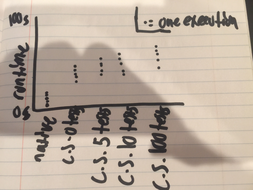
\includegraphics[scale=.75]{images/performance.png}}
        \caption{\emph{This shows the run time difference between the
native program and CrashSimulator in seconds.  Each dot indicates an
        execution.  The X axis shows time values for native executions, and
        executions under CrashSimulator with 0, 5, 10, and 100 tests
        performed respectively.
}}
         \label{figure:performance}

    \end{figure}


{\bf Findings.} Overall, the performance of CrashSimulator is usually
about an order of magnitude slower than if the original program is executed
natively.  It should be noted that in most cases
this slowdown is somewhat mitigated by CrashSimulator's ability to process
tests asynchronously and in other situations it will be more efficient than
running the program natively since {\tt rr's} replay does not require
actual execution of most system calls.  This means that CrashSimulator
avoids the system call overheads, such as I/O.
Even without these improvements, CrashSimulator's runtime is insignificant
compared to the value it offers. During this examination, a single replay
resulted in YYY tests finding ZZZ bugs
(already included in Table~\ref{table:unexpectedtypes}).
Given this success, the longer runtime is worth the wait.
